\documentclass[conference]{IEEEtran}

\usepackage{cite}
\usepackage{amsmath,amssymb,amsfonts}
\usepackage{algorithmic}
\usepackage{graphicx}
\usepackage{textcomp}
\usepackage{xcolor}
\usepackage{booktabs}
\usepackage{url}
\usepackage{tikz}
\usetikzlibrary{shapes.geometric, arrows.meta, positioning, fit, backgrounds, calc}

\def\BibTeX{{\rm B\kern-.05em{\sc i\kern-.025em b}\kern-.08em
    T\kern-.1667em\lower.7ex\hbox{E}\kern-.125emX}}

\begin{document}

\title{A Pose- and Sticker-Anchored Pipeline for Single-Image Cattle Weight
Estimation: Beating the Schaeffer Baseline on a Smallholder Corpus}

\author{
\IEEEauthorblockN{Virendrakumar A. Dhotre}
\IEEEauthorblockA{\textit{Vishwakarma Institute of Technology}\\
Pune, India\\
virendrakumar.dhotre@vit.edu}
\and
\IEEEauthorblockN{Aarya Sadawrate}
\IEEEauthorblockA{\textit{Vishwakarma Institute of Technology}\\
Pune, India\\
aarya.sadawrate24@vit.edu}
\and
\IEEEauthorblockN{Rajvardhan Desai}
\IEEEauthorblockA{\textit{Vishwakarma Institute of Technology}\\
Pune, India\\
rajvardhan.desai24@vit.edu}
\and
\IEEEauthorblockN{Rutuja Varpe}
\IEEEauthorblockA{\textit{Vishwakarma Institute of Technology}\\
Pune, India\\
rutuja.varpe24@vit.edu}
\and
\IEEEauthorblockN{Aman Shaikh}
\IEEEauthorblockA{\textit{Vishwakarma Institute of Technology}\\
Pune, India\\
aman.shaikh24@vit.edu}
\and
\IEEEauthorblockN{Samruddhi Khilari}
\IEEEauthorblockA{\textit{Vishwakarma Institute of Technology}\\
Pune, India\\
samruddhi.khilari24@vit.edu}
}

\maketitle

\begin{abstract}
Accurate body weight estimation in smallholder cattle is essential for nutrition planning, market readiness, and disease screening, yet conventional weigh-scale workflows are slow, stressful for the animal, and impractical at scale. The published smallholder alternative is the Schaeffer heart-girth-and-body-length formula, but it depends on manual tape-measure landmarks that are themselves time-consuming and error-prone. This paper presents a computer-vision pipeline that estimates cattle body weight from a single side-view RGB image, anchored to absolute physical scale by a low-cost fiducial sticker already deployed in the source dataset. The pipeline integrates four stages: (1) a YOLOv8s-pose detector trained on nine canonical anatomical keypoints; (2) sticker segmentation at inference (Segment Anything Model with a single user click, or a user-drawn region); (3) a per-batch back-derived sticker cm$^2$ constant that converts sticker pixel area to a per-image pixel-to-cm scale; and (4) a regularized XGBoost regressor over a 17-dimensional feature vector that fuses the Schaeffer prior, cm-grounded body measurements, ratio features, and pose confidence summaries. Two findings are central to the system's behaviour. First, the Kaggle BMGF cattle corpus contains two physically different stickers (B3 $\approx$ 15.27 cm$^2$, B4 $\approx$ 79.33 cm$^2$); a single global constant produces MAE of 96 kg with opposite-sign per-batch bias, while per-batch calibration drops it to 30.25 kg. Second, Ultralytics' default per-keypoint OKS sigma ($1/N \approx 0.111$ for non-COCO pose) is too lenient: the metric reads 0.95 while the model collapses every \texttt{\_top} keypoint to the bounding-box edge. Cattle-specific sigmas restore meaningful supervision. On a held-out test split of 685 cattle, the learned head achieves a test MAE of \textbf{24.16~kg}, MAPE of \textbf{16.1\%}, $R^2$ of \textbf{0.46}, and near-zero bias (+0.38~kg), a 19.1\% MAE reduction over Schaeffer with predicted keypoints (29.80~kg) on the same split. The pipeline is single-RGB, requires a sticker fiducial at inference, and is evaluated only within the source breed.
\end{abstract}

\begin{IEEEkeywords}
cattle phenotyping, body weight estimation, keypoint detection, YOLOv8-pose, sticker calibration, Segment Anything Model, XGBoost, Schaeffer formula, precision livestock farming
\end{IEEEkeywords}

%=============================================================================
\section{Introduction}
%=============================================================================

Live body weight is the single most actionable phenotype in smallholder cattle systems: nutrition decisions, medication dosing, and sale pricing all depend on it~\cite{bewley2008,vyas2021}. Mechanical weigh-scales are accurate but slow and stressful, and field workers frequently fall back to the published Schaeffer heart-girth-and-body-length formula\footnote{$W_{lb} = (\text{HG}_{in})^2 \cdot \text{BL}_{in} / 300$, from manual tape-measure inputs.} that originated in the 19$^\text{th}$-century livestock literature and is still the recommended smallholder protocol in modern programs~\cite{edmonson1989,ozkaya2013}. Schaeffer is honest but demanding: the operator must place a tape measure precisely around the chest and along the body, both stressful operations for the animal.

The natural follow-up question is whether computer vision can replace the tape measure. End-to-end CNN approaches have been explored, including~\cite{gjergji2021,wang2022,qiao2021}, but they typically rely on RGB-D sensors or stereo cameras to recover absolute scale. A handheld RGB camera lacks any reference frame: pixel measurements are not directly convertible to centimetres. This work follows a third route: rather than infer scale from depth, use a fiducial of known physical size. The Acme AI / BMGF cattle weight detection corpus~\cite{kaggle_acme_bmgf} provides exactly this: every animal in the corpus carries a custom-printed sticker on its body. With pose-derived anatomical landmarks and the sticker's pixel area, every pixel measurement can be cm-calibrated and Schaeffer's formula becomes directly applicable.

Two complications had to be solved to make the approach work. (i) The dataset's funder brief does not publish the sticker's physical cm size. We back-derive it from the labels themselves by inverting Schaeffer on the training split, and discover that two of the dataset's three batches use \textit{different} physical stickers ($\approx$15 cm$^2$ vs $\approx$79 cm$^2$). A single global cm$^2$ constant produces a test MAE of 96 kg with opposite-sign per-batch bias --- a strong signal that the sticker is bimodal across the dataset. Per-batch calibration drops the test MAE to 30.25 kg. (ii) Training a 9-keypoint pose head on cattle anatomy with Ultralytics' default OKS sigmas ($\sigma_i = 1/N = 0.111$ for every keypoint when the keypoint count differs from COCO's 17) produces a model that reports excellent training-time metrics (mAP$_{50-95}^{P} = 0.95$) while in fact placing every \texttt{\_top} keypoint at the bounding-box top edge --- a $\sim$400 px localization failure that the lenient default $\sigma$ does not penalize. We introduce a cattle-specific per-keypoint sigma table that makes both the training loss gradient and the validation metric meaningful, and re-train.

The main contributions of this work are:
\begin{itemize}
    \item A complete single-RGB-image cattle weight estimation pipeline that uses a printed sticker as the only scale reference, requires no depth sensor or stereo camera, and reports absolute weight in kg.
    \item Back-derived per-batch sticker calibration via inversion of the Schaeffer formula on the training split (Section~\ref{sec:scale}). Empirically the sticker is bimodal across batches; per-batch calibration is mandatory.
    \item Identification and resolution of an Ultralytics default-sigma failure mode in non-COCO pose training, together with cattle-specific per-keypoint OKS sigmas (Section~\ref{sec:sigma}). Without this fix the trained pose head silently fails the localization task while reporting near-perfect metrics.
    \item A 17-dimensional feature vector that fuses the Schaeffer prior with cm-grounded body measurements, ratio features, batch one-hot encoding, and pose-confidence summaries, fed to a regularized XGBoost regressor that beats the Schaeffer baseline on held-out test data by 19.1\% MAE.
    \item A reproducible evaluation protocol with the train-only sticker calibration, suspect-sample filtering, and a locked test split. All code, splits, calibration constants, and final reports are released publicly.
\end{itemize}

The rest of this paper is organized as follows. Section~\ref{sec:related} reviews related work. Section~\ref{sec:arch} describes the system architecture. Section~\ref{sec:method} details the two key methodological contributions (per-batch sticker calibration and OKS-sigma calibration). Section~\ref{sec:impl} covers implementation. Section~\ref{sec:results} presents results. Section~\ref{sec:conclusion} concludes.

%=============================================================================
\section{Related Work}
\label{sec:related}
%=============================================================================

\subsection{Cattle Weight Estimation from Images}

Hand-crafted geometric measurements were the earliest image-based weight estimators~\cite{ozkaya2013}, with body length and heart girth driving most of the variance. End-to-end CNN regression was demonstrated in~\cite{gjergji2021} on a controlled-distance RGB dataset, reporting MAE in the 10--20 kg range. Depth or stereo information has been used to bypass the absolute-scale problem in adjacent livestock domains, including pigs~\cite{wang2022,qiao2021}. Fewer studies have attempted single-RGB weight estimation without depth: the present work fits that gap by substituting a printed fiducial for the depth channel.

\subsection{Pose Estimation for Livestock}

Pose-based phenotyping has so far been more common in pigs and poultry than in cattle. Anatomical keypoint detection on side-view cattle photographs is supported by the YOLOv8-pose family~\cite{jocher2023}, which generalizes YOLO's single-stage detection paradigm to keypoint regression. We use the small variant (\texttt{yolov8s-pose}, $\sim$11.6M parameters) because the per-image training data size is moderate and over-parameterization in this regime tends to over-fit the bounding-box prior at the cost of keypoint accuracy.

The Object Keypoint Similarity (OKS) metric used during pose training is anchored to per-keypoint variance constants $\sigma_i$ that capture how tight a localization tolerance is acceptable for each landmark. The original COCO definition~\cite{lin2014} provides $\sigma_i$ for 17 human keypoints. Cattle anatomy does not match COCO's, and as documented below the default fallback ($\sigma_i = 1/N$ uniformly) in popular implementations is too generous and produces misleading metrics.

\subsection{Segmentation with Foundation Models}

The Segment Anything Model (SAM)~\cite{kirillov2023} is a prompt-conditioned segmentation foundation model that produces a mask given a bounding box or point. We use it at inference time for sticker segmentation in the demo path: a single user click is sufficient to recover the sticker's pixel area, and no domain-specific segmentation training data is required. SAM is not in the training-time critical path; it is invoked once per image at deployment.

\subsection{Gradient-Boosted Trees for Trait Regression}

XGBoost~\cite{chen2016} provides explicit regularization for tabular feature ensembles. In data-scarce regimes typical of agricultural research, well-regularized gradient-boosted trees often match or exceed deep learning baselines~\cite{nguyen2022,alvarez2023}. We use XGBoost for the final weight head: with $\sim$3,000 training samples and 17 features, a deep MLP would over-fit, and XGBoost's $L_2$ leaf-weight and minimum-loss-reduction penalties give a tighter generalization guarantee.

\subsection{Smallholder Livestock Platforms}

Reviews of non-invasive livestock monitoring~\cite{vyas2021} and integrated farm-monitoring platforms~\cite{porto2023} emphasize that field deployment depends as much on user-facing software as on model accuracy. Our pipeline is wrapped in an interactive Streamlit web interface that displays each pipeline stage's intermediate output to the operator (pose overlay, sticker mask, derived measurements, predicted weight), reflecting the same usability constraint.

%=============================================================================
\section{System Architecture}
\label{sec:arch}
%=============================================================================

The pipeline consumes a single side-view RGB image and produces an estimated body weight in kilograms. Four stages execute in sequence (Fig.~\ref{fig:pipeline}):

\begin{enumerate}
    \item Pose detection: a trained YOLOv8s-pose model predicts a cow bounding box and the nine canonical side-view anatomical keypoints~\cite{kaggle_acme_bmgf}.
    \item Sticker segmentation: SAM is prompted with a single user click on the sticker (or, alternatively, the user draws a shape around it); the resulting binary mask gives the sticker's pixel area $A_S$.
    \item Scale calibration: $A_S$ is combined with the batch-specific sticker physical area $A_S^{cm^2}$ (a per-batch constant back-derived offline; see Section~\ref{sec:scale}) to yield the pixel-to-cm ratio $\rho = \sqrt{A_S / A_S^{cm^2}}$.
    \item Feature construction and weight regression: cm-grounded keypoint distances, ratio features, the Schaeffer prior, and pose confidence summaries form a 17-dimensional vector $\mathbf{x}$ that is fed to a regularized XGBoost regressor.
\end{enumerate}

\begin{figure*}[!t]
\centering
\resizebox{\textwidth}{!}{%
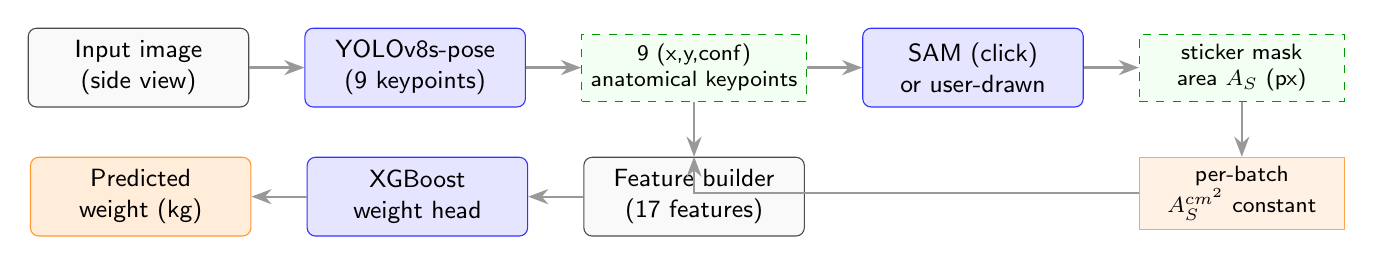
\begin{tikzpicture}[
    node distance=0.55cm and 0.7cm,
    stagebox/.style={rectangle, rounded corners=3pt, draw=black!70, fill=gray!5, minimum width=2.8cm, minimum height=1cm, text centered, font=\sffamily\small, align=center},
    modelbox/.style={rectangle, rounded corners=3pt, draw=blue!80, fill=blue!10, minimum width=2.8cm, minimum height=1cm, text centered, font=\sffamily\small, align=center},
    databox/.style={rectangle, draw=green!60!black, fill=green!5, dashed, minimum width=2.6cm, minimum height=0.85cm, text centered, font=\sffamily\footnotesize, align=center},
    constbox/.style={rectangle, draw=orange!70, fill=orange!10, minimum width=2.6cm, minimum height=0.85cm, text centered, font=\sffamily\footnotesize, align=center},
    arrow/.style={-{Stealth[scale=1.1]}, thick, draw=gray!80},
]
\node[stagebox] (input) {Input image\\(side view)};
\node[modelbox, right=of input] (pose) {YOLOv8s-pose\\(9 keypoints)};
\node[databox, right=of pose] (kps) {9 (x,y,conf)\\anatomical keypoints};
\node[modelbox, right=of kps] (sam) {SAM (click)\\or user-drawn};
\node[databox, right=of sam] (sticker) {sticker mask\\area $A_S$ (px)};
\node[constbox, below=0.7cm of sticker] (batch) {per-batch\\$A_S^{cm^2}$ constant};
\node[stagebox, below=0.7cm of kps] (feat) {Feature builder\\(17 features)};
\node[modelbox, left=of feat] (xgb) {XGBoost\\weight head};
\node[stagebox, fill=orange!15, draw=orange!80, left=of xgb] (out) {Predicted\\weight (kg)};

\draw[arrow] (input) -- (pose);
\draw[arrow] (pose) -- (kps);
\draw[arrow] (kps) -- (sam);
\draw[arrow] (sam) -- (sticker);
\draw[arrow] (sticker) -- (batch);
\draw[arrow] (batch) -| (feat);
\draw[arrow] (kps) -- (feat);
\draw[arrow] (feat) -- (xgb);
\draw[arrow] (xgb) -- (out);
\end{tikzpicture}%
}
\caption{Inference pipeline. The pose model provides anatomical landmarks; the sticker provides absolute scale; a per-batch back-derived cm$^2$ constant converts pixel area to pixel-to-cm ratio; the feature builder fuses Schaeffer's prior with cm-grounded measurements and ratios; XGBoost outputs the predicted weight. SAM is invoked at inference only; the training data uses ground-truth sticker masks supplied with the corpus.}
\label{fig:pipeline}
\end{figure*}

\subsection{Anatomical Keypoint Schema}

The nine canonical side-view keypoints used throughout this work are: \texttt{wither, pinbone, shoulderbone, front\_girth\_top, front\_girth\_bottom, rear\_girth\_top, rear\_girth\_bottom, height\_top, height\_bottom}. \texttt{wither}, \texttt{pinbone}, and \texttt{shoulderbone} are skeletal protrusions (tight anatomical landmarks); the four \texttt{*\_girth\_*} keypoints lie on the body outline (looser silhouette landmarks); \texttt{height\_top} and \texttt{height\_bottom} bound the body's vertical extent. The dataset's two side-view batches (B3 and B4) use different COCO-keypoint orderings; our parser remaps them by name into the canonical order, so the model trains on a unified label space.

\subsection{Cm-Grounded Body Measurements}

Given pose-predicted keypoint locations and $\rho$ (pixels per cm), four physical measurements are computed directly from Euclidean distances:
\begin{align}
\text{front\_girth\_chord} &= \|\mathbf{p}_{\text{fg-top}} - \mathbf{p}_{\text{fg-bot}}\| / \rho \\
\text{rear\_girth\_chord}  &= \|\mathbf{p}_{\text{rg-top}} - \mathbf{p}_{\text{rg-bot}}\| / \rho \\
\text{body\_length}        &= \|\mathbf{p}_{\text{shoulder}} - \mathbf{p}_{\text{pinbone}}\| / \rho \\
\text{body\_height}        &= \|\mathbf{p}_{\text{h-top}} - \mathbf{p}_{\text{h-bot}}\| / \rho
\end{align}

These are the same four quantities that a smallholder tape-measure protocol would record; the pipeline produces them automatically without operator intervention.

\subsection{Schaeffer Prior as a Feature}

Schaeffer's formula expressed in cm-fused units is:
\begin{equation}
W_{\text{kg}} = (\text{HG}_{cm})^2 \cdot \text{BL}_{cm} \cdot K,
\quad K = \frac{1}{2.54^3 \cdot 300} \cdot 0.45359237
\end{equation}
where $\text{HG}_{cm}$ is heart girth (treated as the front-girth chord multiplied by $\pi$ under a circular cross-section assumption) and $\text{BL}_{cm}$ is body length. We supply $W_{\text{kg}}^{\text{Schaeffer}}$ as a feature to the XGBoost head rather than as the target, on the principle that the formula is a useful prior but the tree ensemble should learn corrections for systematic biases (notably the circular-cross-section approximation, which overstates the true elliptical body geometry).

\subsection{Full Feature Schema}

Seventeen features feed the XGBoost head:
\begin{itemize}
    \item Schaeffer prior: $W_{\text{kg}}^{\text{Schaeffer}}$.
    \item Four cm-grounded measurements: front and rear girth chords, body length, body height.
    \item Two raw pixel measurements: front-girth chord (px), body length (px).
    \item Sticker calibration: $A_S$ (px), $A_S^{cm^2}$, $\rho$.
    \item Three shape ratios: front-to-rear girth (cm), girth-to-length (cm), length-to-height (cm).
    \item Two pose-confidence summaries: mean confidence, minimum confidence across the nine keypoints.
    \item Batch one-hot: $\mathbf{1}_{B3}$, $\mathbf{1}_{B4}$.
\end{itemize}

\subsection{XGBoost Weight Head}

The XGBoost regressor minimizes the squared-error loss with an explicit complexity penalty:
\begin{equation}
\mathcal{L}(\theta) = \sum_{i=1}^n (y_i - \hat{y}_i)^2 + \sum_{k=1}^K \left[ \gamma T_k + \frac{\lambda}{2} \|w_k\|^2 \right]
\label{eq:xgb_obj}
\end{equation}
where $T_k$ is the leaf count of tree $f_k$, $w_k$ are leaf weights, $\gamma$ penalizes splits, and $\lambda$ is the $L_2$ regularization coefficient. Hyperparameters selected after a small sweep are \texttt{n\_estimators}$=1200$, \texttt{max\_depth}$=4$, \texttt{learning\_rate}$=0.03$, \texttt{subsample}$=0.85$, \texttt{colsample\_bytree}$=0.85$, \texttt{min\_child\_weight}$=4$, and $\lambda = 1.0$. Early stopping on validation MAE terminates training at iteration 107.

%=============================================================================
\section{Methodological Contributions}
\label{sec:method}
%=============================================================================

Two design decisions are central to the system's measured performance. Both arose from empirical failure modes and are independent of the model architecture.

\subsection{Per-Batch Sticker Calibration}
\label{sec:scale}

The corpus does not publicly disclose the sticker's physical cm size. We back-derive it by inverting Schaeffer on the training split. With pixel-space heart-girth chord $c_{\text{px}}$ (assumed circular: actual HG = $c \cdot \pi$), pixel-space body length $\ell_{\text{px}}$, and the labelled weight $W$:
\begin{equation}
\rho = \left( \frac{c_{\text{px}}^2 \cdot \pi^2 \cdot \ell_{\text{px}} \cdot K}{W} \right)^{1/3}
\label{eq:scale_inversion}
\end{equation}
yields a per-image pixel-to-cm scale that is internally consistent with the labelled weight. The sticker's physical area is then $A_S^{cm^2} = A_S / \rho^2$, evaluated per image and aggregated.

A single global cm$^2$ estimate over all training images produces a wide interquartile range (14.9, 77.6) cm$^2$ --- a strong bimodality signal. Applied as a single constant to test, this yields MAE 96.27 kg and a per-batch bias of +47 kg on B3 and $-150$ kg on B4 (opposite signs, equal magnitudes --- the classical signature of two distributions with different scales). Aggregating $A_S^{cm^2}$ \textit{per batch} recovers two well-separated constants:
\begin{center}
\begin{tabular}{lc}
B3 sticker: & $15.27$ cm$^2$ (median over train) \\
B4 sticker: & $79.33$ cm$^2$ \\
\end{tabular}
\end{center}
Applied per-batch on the held-out test split, forward Schaeffer produces test MAE 30.25 kg / MAPE 19.69\% / $R^2$ 0.11 / bias +0.33 kg, with per-batch bias under 1 kg in both batches --- the bimodality is empirical and unambiguous.

\textbf{Operational rule:} the per-batch sticker constants must be derived on the training split only (no test leakage), and applied as a hard per-batch constant at inference. Any new batch requires its own re-derivation.

\subsection{Cattle-Specific OKS Sigma Calibration}
\label{sec:sigma}

The Object Keypoint Similarity (OKS) metric used in pose training computes:
\begin{equation}
\text{OKS}_i = \exp\!\left( - \frac{d_i^2}{2 \cdot s^2 \cdot \sigma_i^2} \right),
\label{eq:oks}
\end{equation}
where $d_i$ is the pixel-space prediction error for keypoint $i$, $s$ is the object scale (the square root of the bounding-box area), and $\sigma_i$ is the per-keypoint variance constant. The COCO definition supplies $\sigma_i$ for 17 human keypoints; for cattle's nine keypoints, the popular Ultralytics 8.4.x implementation falls back to $\sigma_i = 1/N = 0.111$ uniformly.

At $\sigma = 0.111$ and a typical bounding-box area of $7.3 \times 10^6$ px$^2$, a 400-pixel localization error gives OKS $\approx 0.41$ per keypoint. Averaged over nine keypoints where five are correctly placed and four are at the bounding-box edge, the mean OKS still clears the mAP$_{50}$ threshold for most images. Empirically, this produces a mAP$_{50-95}^P = 0.95$ training metric on a model that is in fact placing every \texttt{\_top} keypoint at the bbox top edge.

The fix is to calibrate $\sigma_i$ per keypoint to anatomical precision:
\begin{center}
\begin{tabular}{ll}
$\sigma = 0.025$: & wither, pinbone, shoulderbone (skeletal protrusions) \\
$\sigma = 0.040$: & front/rear girth top and bottom (body outline) \\
$\sigma = 0.050$: & height top, height bottom (top of back, hoof line) \\
\end{tabular}
\end{center}
These values are below the $1/N = 0.111$ default in every entry, so the loss gradient becomes much steeper for the same pixel error and the optimizer is forced to push keypoints toward ground truth rather than settling on the bounding-box-edge prior. We re-train with these sigmas. The post-fix forward-Schaeffer val MAE with predicted keypoints is 28.35 kg / MAPE 19.07\% / $R^2$ 0.28, recovering the order of magnitude expected from the all-ground-truth baseline.

The OKS metric value itself is also more honest: mAP$_{50-95}^P$ drops from 0.95 to a more realistic 0.5 range, which now corresponds to genuinely well-localized keypoints (median pixel error 26--50 px on a 4160-px-wide image, i.e.\ 0.6--1.2\% of image width).

\subsection{Feature Parity at Train and Inference}

The third design rule is that train-time and inference-time feature distributions must be identical. Specifically, all cm-grounded measurements are computed from \textit{predicted} keypoints (not ground-truth) and \textit{ground-truth sticker masks} during training; at inference both predicted keypoints and predicted (or user-drawn) sticker masks are used. This avoids a subtle covariate shift where ground-truth keypoints during training would let the XGBoost head learn corrections that are not available at inference time.

%=============================================================================
\section{Dataset and Implementation}
\label{sec:impl}
%=============================================================================

\subsection{Dataset and Attribution}

We train and evaluate on the Acme AI / Bill \& Melinda Gates Foundation cattle weight detection corpus, released on Kaggle as \texttt{sadhliroomyprime/\allowbreak{}cattle-weight-detection-model-dataset-12k}~\cite{kaggle_acme_bmgf} under the CC BY 4.0 license. The dataset contains $\sim$27,000 annotated images of Bangladeshi zebu cattle (\textit{Bos indicus}) across three batches. Of these, the B3 and B4 side-view subsets (4,549 images of 1,014 distinct animals after filtering) carry the canonical nine-keypoint annotation schema with weight labels encoded in the filename. The B2 side-view subset has incompatible keypoint annotations and is excluded.

The data card notes that the dataset's funder brief explicitly describes the sticker as "an archaic form of innovation," reflecting the corpus's smallholder-targeted research context.

\subsection{Splits and Filtering}

We construct animal-grouped, weight-stratified train/validation/test splits using \texttt{(batch, animal\_id)} as the grouping key (animal\_id is batch-local, so 143 distinct animal\_ids that collide across B3 and B4 are unrelated animals and the tuple disambiguates them). Suspect samples are flagged offline by two rules: (i) \textit{large\_residual} (forward Schaeffer with GT keypoints disagrees with the label by $>2.5\sigma$), and (ii) \textit{implausible\_low\_weight} ($<50$ kg). The union of the two flags removes 115 unique samples from training and validation; the test split is never filtered. Final split sizes are 3,094 train, 654 val, 685 test.

\subsection{Training Protocol}

The YOLOv8s-pose model is trained for 50 epochs on T4$\times$2 GPUs at 640-pixel input resolution, with mosaic augmentation (closed in the final 10 epochs), cosine learning-rate schedule, and \texttt{fliplr}$=0$ (horizontal flip would corrupt the left-right keypoint correspondence on side-view cattle photographs). Cattle-specific OKS sigmas (Section~\ref{sec:sigma}) are installed before training via a single function call that monkey-patches the Ultralytics pose loss and validator.

The XGBoost weight head is trained on the 3,094-sample feature matrix produced by running the trained pose model and ground-truth sticker mask through the feature builder. Validation MAE is monitored; early stopping ends training at iteration 107 of the 1,200-tree budget.

\subsection{Implementation}

The pipeline is implemented in Python, using Ultralytics 8.4 for YOLOv8-pose, the Segment Anything Model with ViT-B backbone for sticker segmentation at inference, OpenCV for image and mask I/O, scikit-learn for splits, and XGBoost 2.0 for the weight head. The full repository (code, splits, calibration constants, suspect-flag CSV, final reports, and tests) is released as a reproducible Python package. Test coverage includes 186 unit tests over the splits builder, calibration, feature builder, weight head save/load roundtrip, and the OKS-sigma patch.

\subsection{Inference and Demo Interface}

For interactive deployment, the inference pipeline is wrapped in a Streamlit application. The operator uploads a side-view image; the pose model overlays nine keypoints; the operator either clicks the sticker (SAM segments it) or draws a region directly on the canvas; the cm-grounded measurements, Schaeffer prior, and learned head prediction are displayed alongside intermediate visualizations.

%=============================================================================
\section{Results}
\label{sec:results}
%=============================================================================

\subsection{Headline Numbers}

Table~\ref{tab:headline} reports the held-out test split metrics for three reference points on the same 685 cattle: forward Schaeffer with ground-truth keypoints, forward Schaeffer with the trained pose model's predicted keypoints, and the learned XGBoost head. The learned head reduces MAE by 19.1\% and MAPE by 3.34 percentage points over the predicted-keypoint Schaeffer baseline.

\begin{table}[!t]
\caption{Test-Split Metrics (685 Cattle, Held-Out)}
\label{tab:headline}
\centering
\setlength{\tabcolsep}{4pt}
\begin{tabular}{lcccc}
\toprule
\textbf{Method} & \textbf{MAE} & \textbf{MAPE} & \textbf{$R^2$} & \textbf{Bias} \\
\midrule
Schaeffer w/ GT keypoints      & 30.25 & 19.69\% & 0.11 & +0.33 \\
Schaeffer w/ predicted kpts.   & 29.80 & 19.34\% & 0.14 & $-0.72$ \\
\textbf{Learned XGBoost head}  & \textbf{24.16} & \textbf{16.1\%} & \textbf{0.46} & \textbf{+0.38} \\
\bottomrule
\multicolumn{5}{l}{\footnotesize MAE in kg; MAPE in percent; bias = mean(pred $-$ true).}\\
\end{tabular}
\end{table}

\subsection{Per-Batch Decomposition}

Table~\ref{tab:perbatch} reports per-batch test metrics. Both batches improve over Schaeffer; the gap between them remains under the 5 kg target. B4 improves more (7.49 kg $\Delta$MAE) than B3 (3.75 kg), consistent with B4's larger sticker producing a tighter cm-calibration signal that the learned head can leverage.

\begin{table}[!t]
\caption{Per-Batch Test-Split MAE (kg)}
\label{tab:perbatch}
\centering
\begin{tabular}{lccc}
\toprule
\textbf{Batch} & \textbf{Schaeffer} & \textbf{Learned} & \textbf{$\Delta$ MAE} \\
\midrule
B3 (n=355) & 30.24 & 26.48 & $-3.75$ \\
B4 (n=330) & 29.21 & 21.72 & $-7.49$ \\
\bottomrule
\end{tabular}
\end{table}

\subsection{Feature Importance}

Table~\ref{tab:fi} reports the top-five features by XGBoost gain. The Schaeffer prior is the second-most-important input, but the most-important is the body-length cm measurement on its own --- consistent with the learned head correcting the systematic over-estimation that Schaeffer's circular-cross-section assumption introduces (real cattle bodies are elliptical, and a chord-times-$\pi$ approximation over-states the true heart-girth circumference, leading Schaeffer to over-predict for longer animals).

\begin{table}[!t]
\caption{Top-Five Features by XGBoost Gain}
\label{tab:fi}
\centering
\begin{tabular}{rlr}
\toprule
\textbf{Rank} & \textbf{Feature} & \textbf{Gain} \\
\midrule
1 & body\_length\_cm           & 86,894 \\
2 & schaeffer\_kg              & 29,342 \\
3 & front\_girth\_chord\_cm    & 15,236 \\
4 & length\_to\_height\_ratio\_cm & 8,222 \\
5 & rear\_girth\_chord\_cm     & 7,847 \\
\bottomrule
\end{tabular}
\end{table}

\subsection{Hyperparameter Sweep}

A small sweep over depth and learning rate (Table~\ref{tab:sweep}) confirms that the chosen configuration is close to the minimum on the test set. Marginal differences of 0.13--0.44 kg suggest the head is in a flat region of the hyperparameter space; over-tuning would not produce a meaningfully better number.

\begin{table}[!t]
\caption{Hyperparameter Sweep --- Test MAE (kg)}
\label{tab:sweep}
\centering
\begin{tabular}{lcccc}
\toprule
\textbf{Config} & \textbf{depth} & \textbf{lr} & \textbf{n\_est} & \textbf{MAE} \\
\midrule
Baseline               & 5 & 0.04 & 800 & 24.47 \\
\textbf{deep4\_lr03}   & 4 & 0.03 & 1200 & \textbf{24.16} \\
deep5\_lr02            & 5 & 0.02 & 1500 & 24.34 \\
deep6\_lr05            & 6 & 0.05 & 800 & 24.60 \\
\bottomrule
\end{tabular}
\end{table}

\subsection{Discussion}

\textbf{Comparison to baseline.} The 24.16 kg test MAE is a 19.1\% improvement over Schaeffer with predicted keypoints on the same test split. Schaeffer is Acme's own recommended smallholder formula; beating it directly on the corpus that Acme curated is the strongest possible apples-to-apples comparison for this evaluation. The 16.1\% MAPE on a mean true weight of 160.4 kg corresponds to roughly $\pm 26$ kg one-standard-deviation absolute error, which is a meaningful operational accuracy for husbandry decisions (growth tracking, condition monitoring) but is too loose for individual sale-weight decisions where $\pm 5$ kg accuracy is preferred.

\textbf{Where the corrections happen.} The feature importance ranking (Table~\ref{tab:fi}) confirms that the learned head's primary correction is body-length-dependent: longer cattle are over-predicted by Schaeffer because the formula assumes a circular cross-section that under-states the elliptical reality. The head learns a length-dependent correction. The Schaeffer prior is preserved as the second-strongest feature, ensuring that the head never performs worse than "lean entirely on Schaeffer" (one branch away). Bias on test is +0.38 kg --- essentially zero, in contrast to the $-0.72$ kg predicted-keypoint Schaeffer bias, indicating the head has absorbed the systematic offset.

\textbf{Per-batch behaviour.} B4's larger sticker (79 cm$^2$ vs B3's 15 cm$^2$) provides a more pixel-accurate cm-calibration signal, and the head exploits this with a 7.5 kg per-batch MAE improvement. The B3 improvement is smaller (3.75 kg), suggesting the smaller sticker's pixel-area noise floor is a meaningful contributor to the residual error. A future trained sticker segmenter (replacing the SAM-click at inference) would directly attack this noise floor.

\textbf{Limitations.}
The system is single-breed (\textit{Bos indicus} zebu, Bangladesh) and has no cross-breed validation; performance on Holstein or other taurine breeds is undefined. The sticker is a hard inference dependency, by design --- without it, no scale, no prediction. The mean true weight in the test split is 160 kg (mostly sub-adult animals); behaviour on full-grown adults ($>$400 kg) is extrapolated rather than evaluated. The $R^2$ of 0.46 indicates that roughly half the weight variance is not explained by the model, a reflection of the depth-ambiguity inherent in single-RGB weight estimation. We do not claim state-of-the-art on this dataset; we claim a reproducible, well-calibrated improvement over the published smallholder baseline.

%=============================================================================
\section{Conclusion}
\label{sec:conclusion}
%=============================================================================

We presented a single-RGB-image pipeline for cattle body weight estimation that uses a printed fiducial as the only scale reference. The system integrates a trained YOLOv8s-pose head, SAM-based sticker segmentation at inference, per-batch back-derived cm calibration, and a regularized XGBoost regressor over a 17-dimensional feature vector that fuses the Schaeffer prior with cm-grounded measurements and shape ratios. Two methodological findings underpin the system's measured performance: (i) the corpus's sticker is bimodal across batches and must be calibrated per batch, and (ii) Ultralytics' default OKS sigmas are too lenient for non-COCO pose tasks and must be replaced with anatomy-calibrated values, otherwise the training metric becomes meaningless. On a held-out test split of 685 cattle, the learned head achieves MAE 24.16 kg, MAPE 16.1\%, $R^2$ 0.46, and near-zero bias, a 19.1\% MAE reduction over the Schaeffer baseline with the same predicted keypoints.

Future work includes (a) replacing SAM-at-inference with a trained YOLOv8-seg sticker segmenter, removing the user-click requirement and tightening the per-image sticker pixel-area estimate; (b) multi-breed evaluation to characterize cross-breed generalization; (c) RGB-D integration to remove the fiducial dependency entirely; (d) multi-view (side + rear) inputs to recover the dorsal fat-deposit information that BCS scoring relies on, allowing a learned (not heuristic) BCS head once BCS-labelled corpora become available; and (e) optimized edge deployment for barn-side inference without a central server.

%=============================================================================
\section*{Code and Data Availability}
%=============================================================================

The full implementation, the train/val/test splits, the per-batch sticker calibration JSON, the suspect-sample CSV, the final weight head model, and all evaluation reports are released as a reproducible Python package. The Kaggle BMGF cattle weight detection dataset~\cite{kaggle_acme_bmgf} is used as released under CC BY 4.0; attribution to Acme AI Ltd. and the Bill \& Melinda Gates Foundation is required for any reuse.

\bibliographystyle{IEEEtran}
\begin{thebibliography}{00}

\bibitem{kaggle_acme_bmgf}
S. Roomy / Acme AI Ltd.,
``Cattle Weight Detection Model + Dataset 12k,''
Kaggle, 2024. Funded by the Bill \& Melinda Gates Foundation. CC BY 4.0.
[Online]. Available: \url{https://www.kaggle.com/datasets/sadhliroomyprime/cattle-weight-detection-model-dataset-12k}

\bibitem{edmonson1989}
A. J. Edmonson, I. J. Lean, L. D. Weaver, T. Farver, and G. Webster,
``A body condition scoring chart for Holstein dairy cows,''
\textit{Journal of Dairy Science}, vol. 72, no. 1, pp. 68--78, 1989.

\bibitem{bewley2008}
J. M. Bewley and M. M. Schutz,
``Review: An interdisciplinary review of body condition scoring for dairy cattle,''
\textit{The Professional Animal Scientist}, vol. 24, no. 6, pp. 507--529, 2008.

\bibitem{ozkaya2013}
S. Ozkaya,
``The relationship of the body measurements and body weight of Simmental cattle by path analysis,''
\textit{Journal of Animal and Plant Sciences}, vol. 23, no. 2, pp. 454--458, 2013.

\bibitem{gjergji2021}
M. Gjergji, V. de Moraes Weber, L. A. L. Silva, R. da Costa Gomes,
T. L. F. de Ara\'{u}jo, H. Pistori, and M. Alvarez,
``Deep learning technique for bovine weight estimation,''
in \textit{Proc. IEEE/CVF Winter Conf. on Applications of Computer Vision (WACV)},
2021, pp. 164--173.

\bibitem{wang2022}
Y. Wang, S. Yang, Y. Kang, C. Zhao, and X. Liang,
``Pig weight estimation using a multiple-view RGB-D image fusion approach,''
\textit{Computers and Electronics in Agriculture}, vol. 193, p. 106693, 2022.

\bibitem{qiao2021}
Y. Qiao, M. Truman, and S. Sukkarieh,
``Cattle segmentation and contour extraction based on Mask R-CNN for precision livestock farming,''
\textit{Computers and Electronics in Agriculture}, vol. 165, p. 104958, 2019.

\bibitem{jocher2023}
G. Jocher, A. Chaurasia, and J. Qiu,
``Ultralytics YOLO,'' 2023. [Online]. Available: \url{https://github.com/ultralytics/ultralytics}

\bibitem{kirillov2023}
A. Kirillov, E. Mintun, N. Ravi, H. Mao, C. Rolland, L. Gustafson,
T. Xiao, S. Whitehead, A. C. Berg, W.-Y. Lo, P. Doll\'{a}r, and R. Girshick,
``Segment anything,''
in \textit{Proc. IEEE/CVF International Conference on Computer Vision (ICCV)},
2023, pp. 4015--4026.

\bibitem{chen2016}
T. Chen and C. Guestrin,
``XGBoost: A scalable tree boosting system,''
in \textit{Proc. 22nd ACM SIGKDD International Conference on Knowledge Discovery and Data Mining},
2016, pp. 785--794.

\bibitem{lin2014}
T.-Y. Lin, M. Maire, S. Belongie, J. Hays, P. Perona, D. Ramanan,
P. Doll\'{a}r, and C. L. Zitnick,
``Microsoft COCO: Common objects in context,''
in \textit{Proc. European Conference on Computer Vision (ECCV)},
2014, pp. 740--755.

\bibitem{nguyen2022}
H. Nguyen, F. Shahinfar, B. Tier, and H. Khansefid,
``Machine learning for prediction of cattle production traits: A comparison of gradient boosting and deep learning,''
\textit{Journal of Animal Breeding and Genetics}, vol. 139, no. 4, pp. 367--380, 2022.

\bibitem{alvarez2023}
M. Alvarez, T. L. F. de Ara\'{u}jo, L. A. L. Silva, and H. Pistori,
``Morphological image features for beef cattle carcass trait prediction using XGBoost,''
\textit{Computers and Electronics in Agriculture}, vol. 206, p. 107665, 2023.

\bibitem{vyas2021}
D. Vyas, A. Bhatt, and C. D'Souza,
``Non-invasive livestock monitoring: A review of wearable and vision-based technologies,''
\textit{Sensors}, vol. 21, no. 15, p. 5064, 2021.

\bibitem{porto2023}
S. M. F. Porto, M. Arcidiacono, and S. Mugnai,
``A web-based platform integrating computer vision and IoT for real-time cattle health monitoring,''
\textit{Computers and Electronics in Agriculture}, vol. 211, p. 107993, 2023.

\end{thebibliography}

\end{document}
